\section{Requirement and Design}

\subsection{Requirements}
Design phase of the software development involves several crucial processes and one of them is identifying requirements. Requirements must be specified in a clear and unambiguous way in order to guide the team towards the final aim. Taking into account that,  it is not always possible to meet all the requirements in the given time,  prioritising them into different levels is very  beneficial for any software development project.  Software requirements are divided into two major groups: functional requirements and non-functional requirements. Simply, functional requirements determine system functionalities (e.g. what system should do), and non-functional requirements specify the constraints that will be on the system\cite{msads}.

\begin{figure}[h]
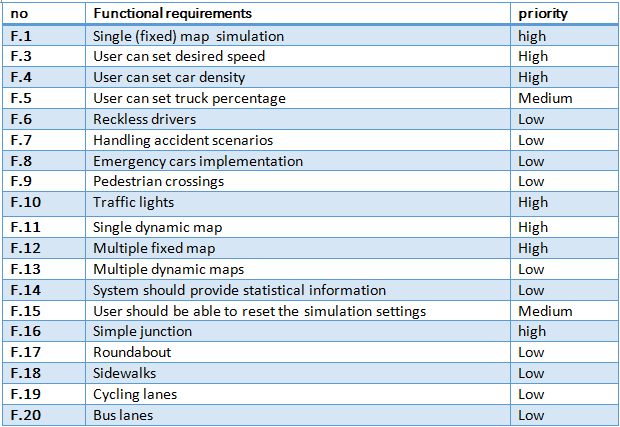
\includegraphics[width=14cm, height=10cm]{pics/FR}
\centering
\caption{Functional Requirements}
\end{figure}

\begin{figure}[H]
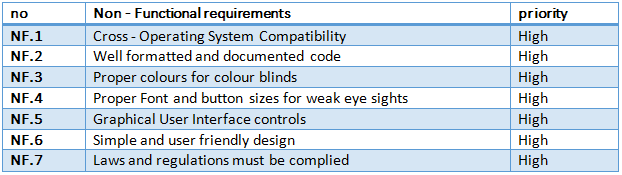
\includegraphics[width=14cm, height=4cm]{pics/NFR}
\centering
\caption{Non-Functional Requirements}
\end{figure}


\subsection{Use Case}

When considering the diagrams to represent system interaction, we see there are variety of them, however not all of them are appropriate for each project. One of the essential diagrams to depict user's interaction with the system is Use Case diagram. Use case diagrams are usually referred to as behaviour diagrams used to describe a set of actions (use cases) that some system or systems (subject) should or can perform in collaboration with one or more external users of the system (actors)\cite{umlucd}.\newline
 
\begin{figure}[H]
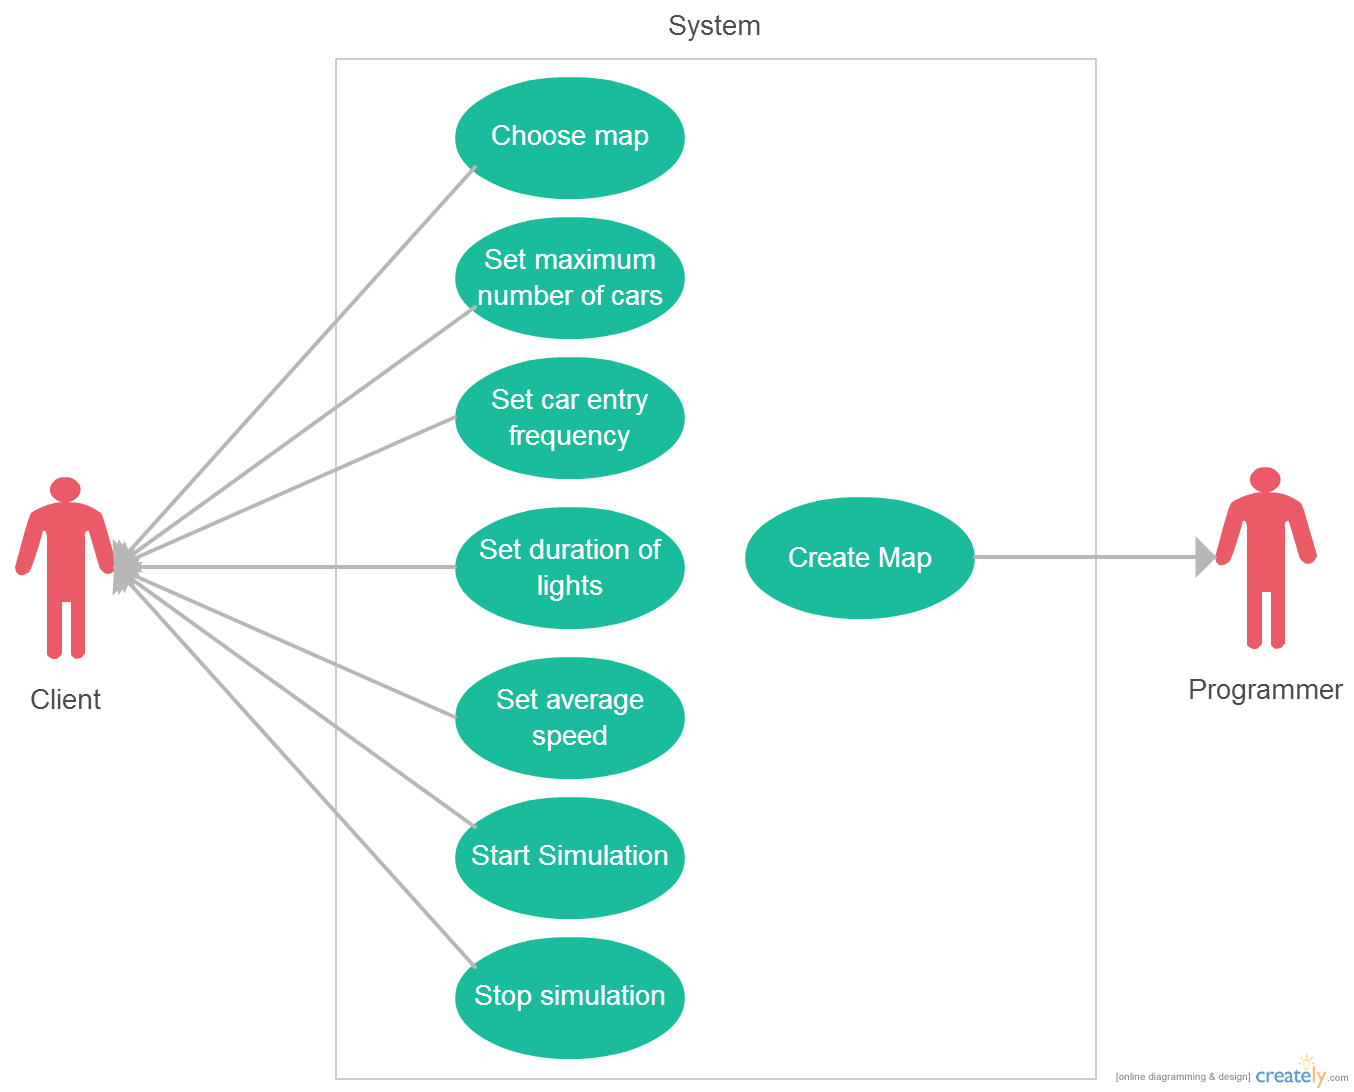
\includegraphics[width=12cm, height=12cm]{pics/useCase}
\centering
\caption{Traffic Simulation Use Case}
\end{figure}

\subsection{Software Development Methodology}
\indent There is a plethora of systems development methodologies, each with differing strengths, weaknesses and target industries. A well-known and traditional methodology used to develop and maintain IT systems is the Systems Development Lifecycle (SDLC) \cite{hoff}. One of the earliest and most established expressions of the SDLC is the waterfall model \cite{Sch95}. The waterfall model can be convenient for certain project because it has been adopted by many and different types of projects and due to some of its advantages. For instance, it recommends a linear approach to software construction, which allows stakeholders to easily understand the processes involved. \newline

\indent However, it also has some issues that need to be taken into consideration when developing IT projects. For example, the project is committed to a frozen set of detailed requirements \cite{larm}, which makes it very difficult to adapt, in case extra requirements are to be added at later stages. What is more, each phase is independent and developed over a fairly long period of time and they cannot be revisited once complete. Large steps are taken in which many decisions are made without the benefit of concrete feedback from realistic implementation and testing \cite{larm}.
 
\subsection{Iterative and Incremental development}
\indent On the other hand, there are other methodologies, such as, the Iterative model, which can be more suitable for certain types of projects. According to Larman, 2005 \cite{larm}, the Iterative development offers support to reduce some problems exacerbated by a linear waterfall model. The Iterative approach consists mainly in developing in short periods of time, providing constant feedback and allowing adaptation \cite{larm}.  This approach has four phases. These are inception, elaboration, construction and transition. Within each phase, there are five disciplines: requirements, analysis, design, implementation (building the software) and test\cite{cadle}. Figure 5 explains how development is none using this models.
 
\begin{figure}[H]
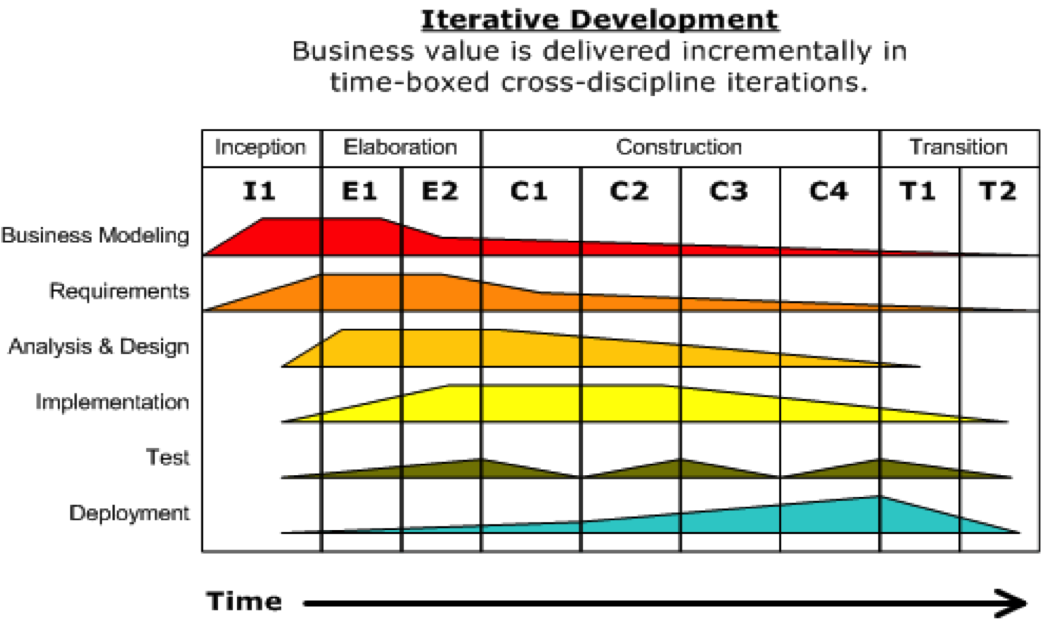
\includegraphics[width=12cm, height=8cm]{pics/methodology}
\centering
\caption{Iterative and Incremental development model}
\end{figure}
 
 In contrast to the waterfall model, in this approach, development is done into a series of short, fixed-length (for example, four week) mini-projects called iterations; the outcome of each is a tested, integrated, and executable system\cite{larm}. These characteristics of this approach were more reflected to our project needs and hence we selected it over the waterfall. We started to develop immediately, after obtaining the system specifications. We decided not to concentrate so much time, in only one particular process, analyzing or designing the system, for example. Instead, we opted to start working on several processes in parallel in order to have some early and visible results of the traffic simulation. \newline
 
\indent Furthermore, we have decided to address the problem in this way, because of the two types of requirements that we aimed to achieve. We defined primary requirements, which were fixed, and secondary requirements, which were evolving over the weeks. Hence, we needed to use a model, such as the Iterative one, that could adapt to our project, and that allowed us to make changes to the requirements, which eventually triggered modifications to the whole system, including the designs, coding and testing. Further advantages\cite{larm} that encouraged us using this approach are summarized bellow:
 
\begin{enumerate}[itemsep=1pt]
\item Risk mitigation: Early rather than late mitigation of high risks (technical, requirements, objectives, usability, and so forth)
\item Agility: Early feedback, user engagement, and adaptation, leading to a refined system that more closely meets the real needs of the stakeholder
\item Managed complexity: The team is not overwhelmed by "analysis paralysis" or very long and complex step
\item Guidance: Early visible progress
\end{enumerate}

%Should this be as a new section or subsection-------------------------
\newpage
%Should this be as a new section or subsection
\section{Back End Design}

\indent The above section described the design for the user interaction for the front end of the software, the following section will cover the design and construction of the simulation. 

\subsection{Constructing the Map}

\indent In the context of the simulation, the game board can be defined as the area in which the siulation is presented. A more precise definition, our game board can be represented as a two dimentional matrix $ G_{i,j} $ where $ i = 1 \dots m $ and $ j = 1 \dots n $. More specifically, 

\begin{figure}[h]
\centering  
\[ 
G_{m,n} = 
\begin{bmatrix}
    g_{1,1} & g_{1,2} & \cdots & g_{1,n} \\
    g_{2,1} & g_{2,2} & \cdots & g_{2,n} \\
    \vdots  & \vdots  & \ddots & \vdots  \\
    g_{m,1} & g_{m,2} & \cdots & g_{m,n} 
  \end{bmatrix} \]
\end{figure}

In this way, the game board gives us a matrix (a grid) which is used as the foundation for identifying the placement of lanes, lights and agents on the board. 

\subsection{Constructing lanes and Junctions}

\indent Using the game board with variable height and width a natural progression was the designing of the lanes. A lane can be thought of as a line which has a starting and end position. The start and end position must reside within the bounds of the two dimensional matrix. Each element of the matrix corresponds to a point on a lane.   
%Single Lane picture 
\begin{figure}[H]
    \centering
    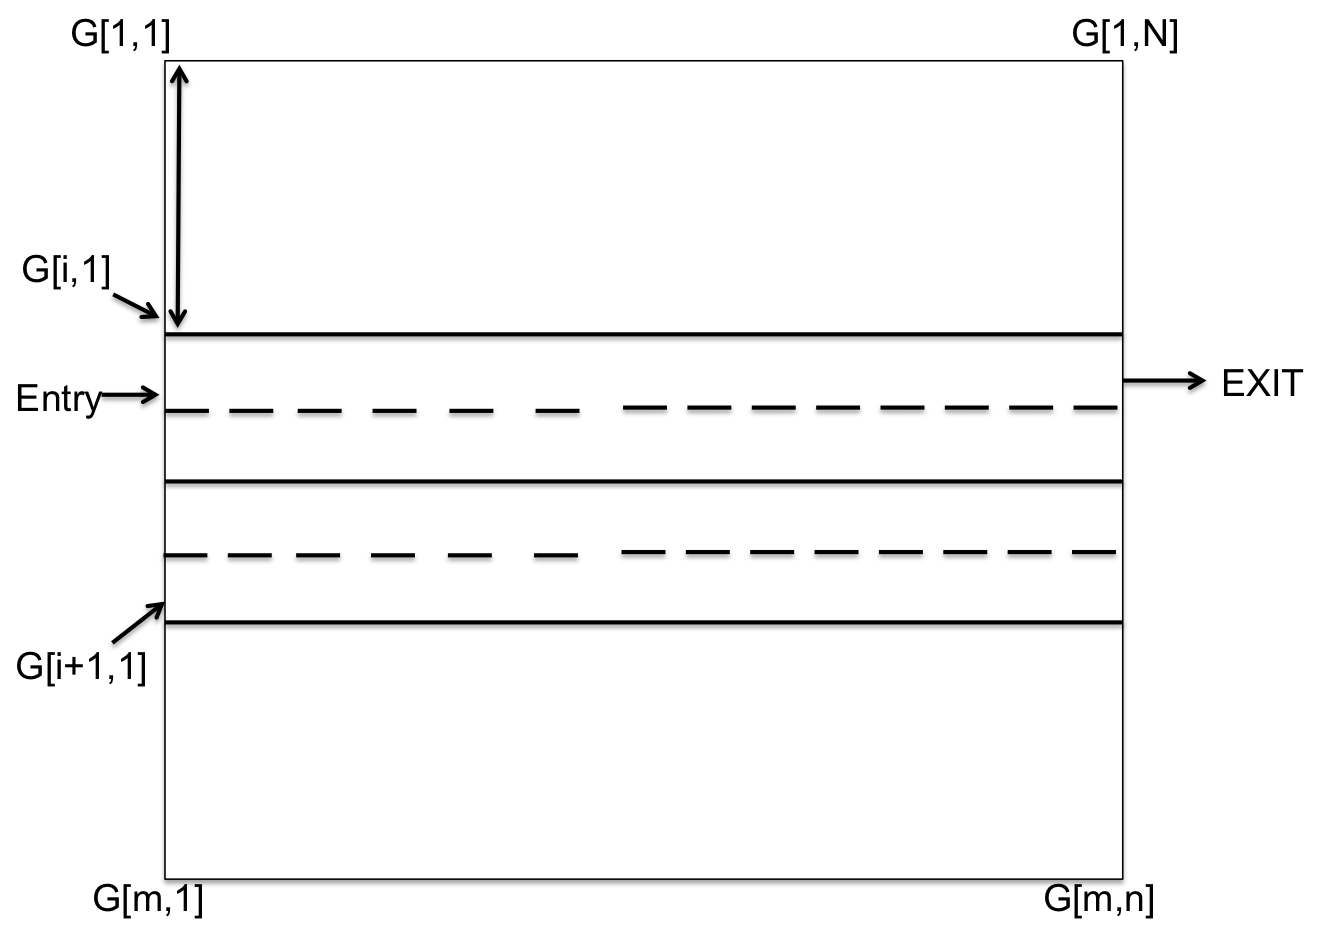
\includegraphics[width=0.8\textwidth]{pics/lane.png}
    \caption{Two lanes on the game board}
    \label{fig:Lanes}
\end{figure}
Figure \ref{fig:Lanes} describes a lane ontop of our game board matrix. \newline
\indent A junction is a crossing of one or more lanes. Each lane has a start and end point. The placement of the junction on our gameboard is as follows. 
%put the junction here 
\begin{figure}[H]
    \centering
    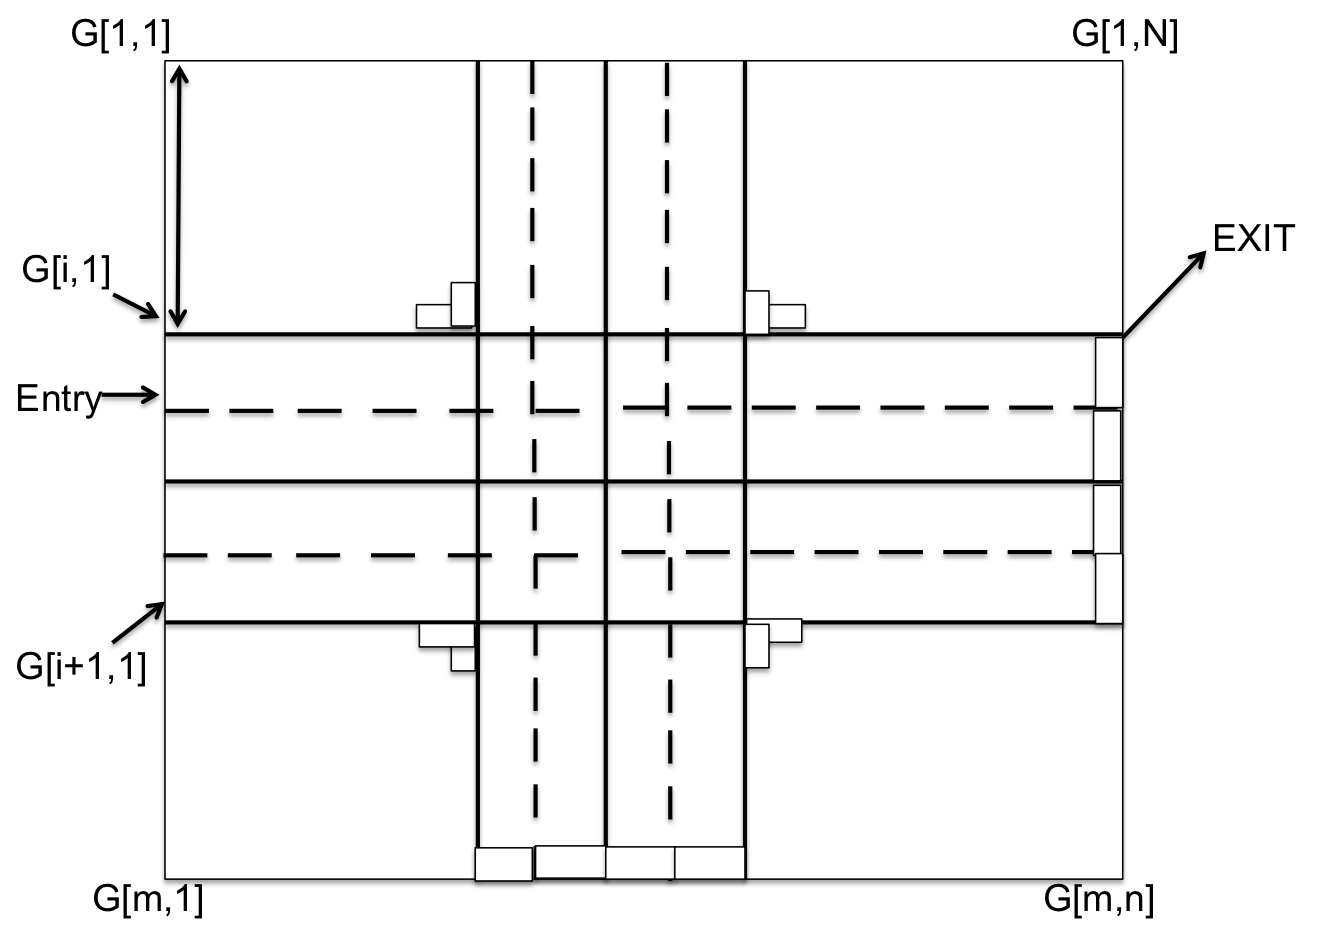
\includegraphics[width=0.8\textwidth]{pics/map.png}
    \caption{Single junction on the Game Board} 
    \label{fig:SingleJunctionPhysical}
\end{figure}
Figure \ref{fig:SingleJunctionPhysical} describes a single junction. The idea of a single junction can be applied to a map with multiple juncitons. Having adressed the construction of the gamebard, lanes and junctions we can move onto the logical components of the lanes and junctions. \newline
\indent Having a designed a physical map we can begin to assign some logical components to it - starting with a single junction consisting of two lanes in the North South East and West directions. Each lane is given an id and direction. The lane id's are odd and even numbers (starting at 1) and the direction of a lane is an integer value ranging from $ 0 \dots 3 $. 
%Logic for map1_1Intersetion
\begin{figure}[H]
    \centering
    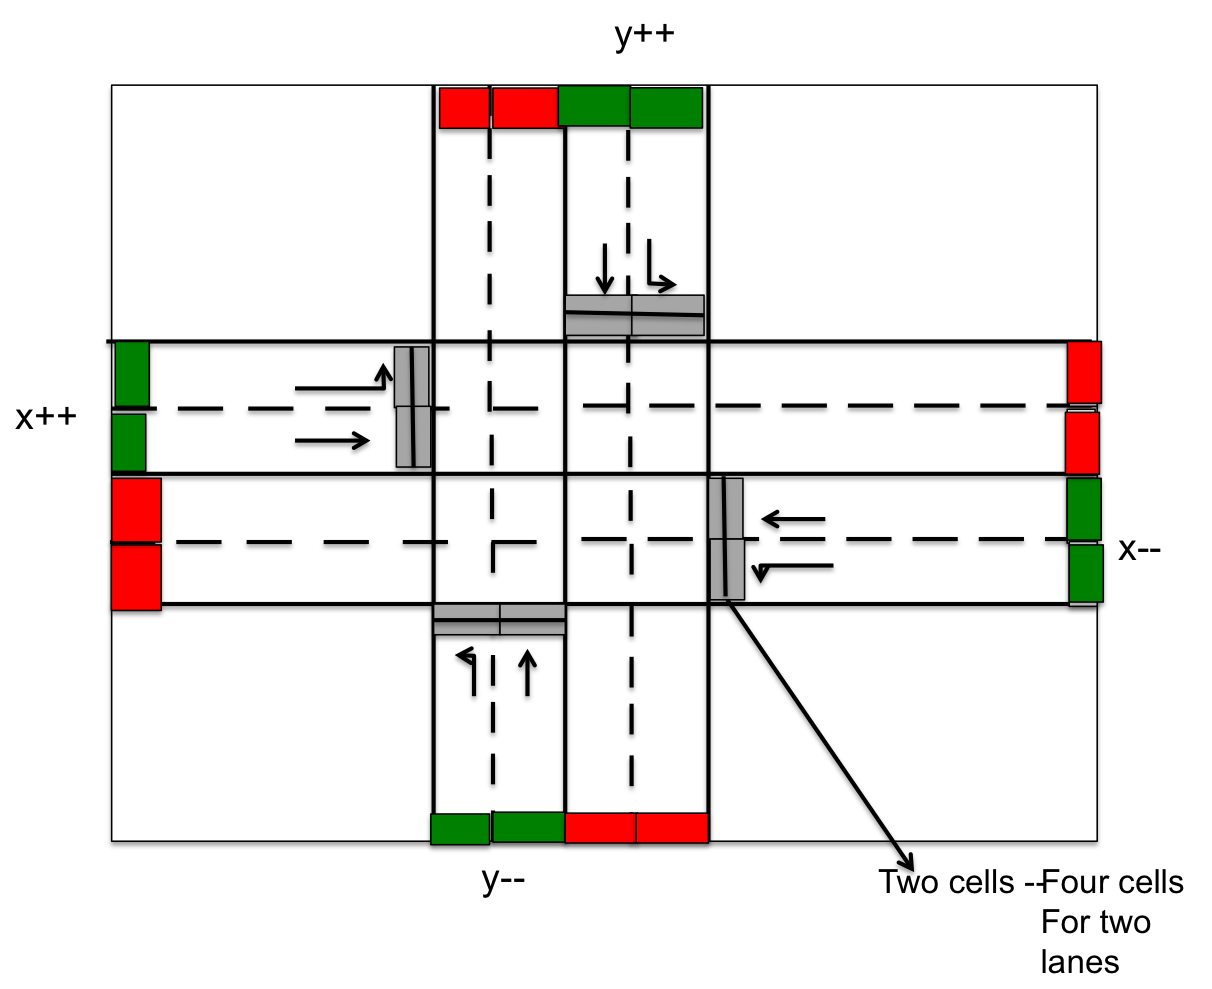
\includegraphics[width=0.8\textwidth]{pics/map2.png}
    \caption{Single junction Logic} 
    \label{fig:SingleJunction}
\end{figure}
In figure \ref{fig:SingleJunction}, a starting cell is given the color green and the end cell red. The lane id and directions are listed to the left of the lanes. The inner most lanes are for vehicles travelling straight hrough a junction and the outer most (odd and even) lanes are for vehicles who will be turning. Using the same logic, this can be applied to a map with the same number of lanes but changing the number of junctions.\newline
%Logic for map2_4Intersetions 
\begin{figure}[H]
    \centering
    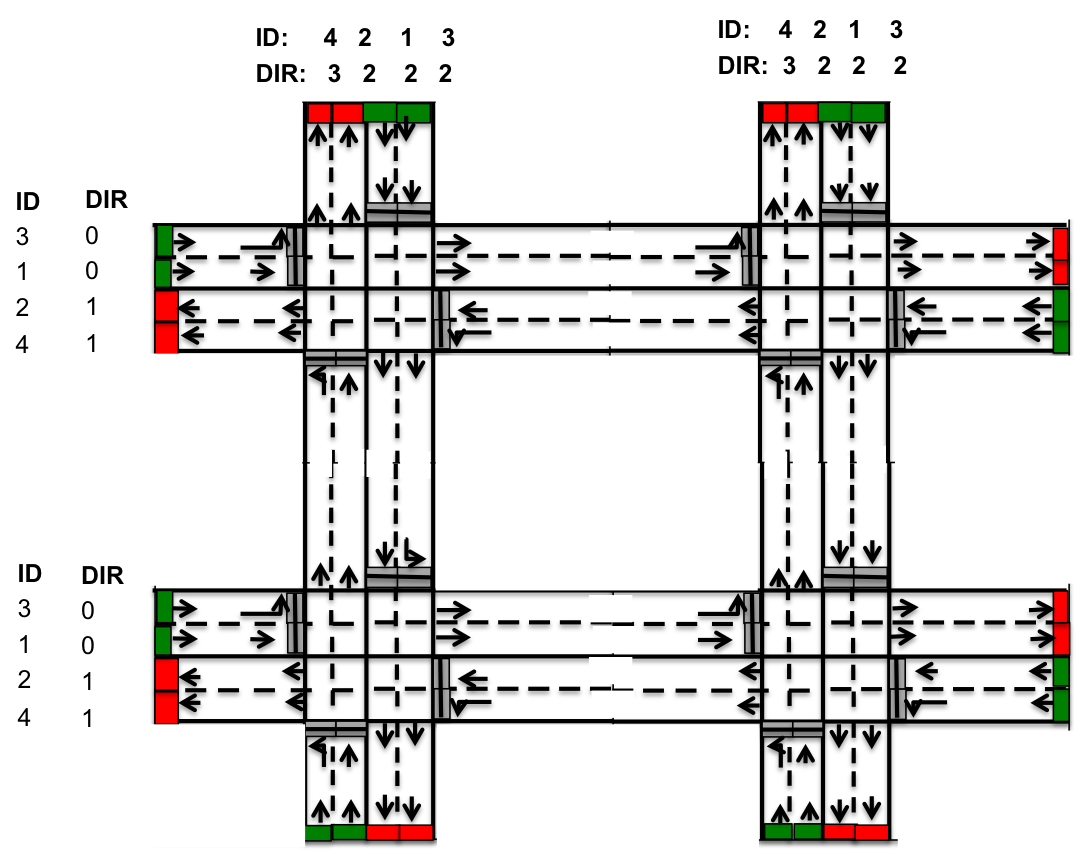
\includegraphics[width=0.8\textwidth]{pics/map3.png}
    \caption{Multijunction lane logic} 
    \label{fig:Multijunction}
\end{figure}

\indent In the same way, a network consisting of multiple lanes and junctions \ref{fig:Multijunction} can be constructed with the same logic used in a grid with a single junction.  


%--------------------------------

\subsection{Class Diagram}
This section explains the class-digram of the entire system. The biggest class is the car class. It has several relations to  other components of the system. However, in the figure bellow, it does not show these links to the respective components, because of page size limitation. Nevertheless, the following explains  briefly, how the Car class is related to the respective classes. 

The class diagram links to the following classes: \texttt{Lane}, \texttt{Cell}, \texttt{Light} and \texttt{Map}.

Finally, the \texttt{GamePanel} class also has an important relation with \texttt{Car} class, as it can have many cars objects. 

\begin{figure}[H]
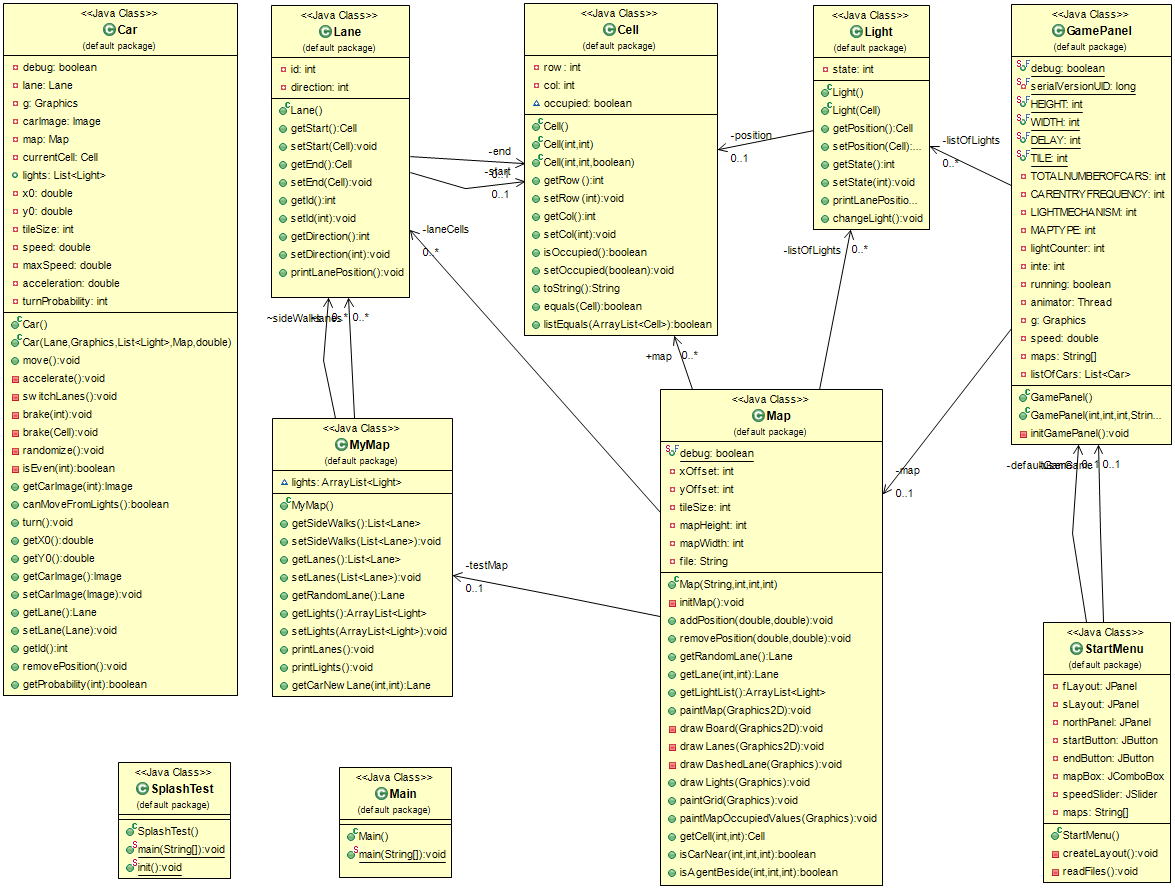
\includegraphics[width=16cm, height=15cm]{pics/classDiagram}
%\centering
\caption{Traffic simulation class diagram}
\end{figure}

